% CAPÍTULO 28 — «O preço da proteção que protege» (andar 1: o que não se compra, fechado pelo outro lado)
% Fracasso que o abre: o mundo mais pesado do capítulo da margem perde \numMargemPerdaRazao{} vez o
% controle sem que a correlação se mexa, e os dias conjuntos vão de \numMargemExcessoControle{} a
% \numMargemExcessoDezPorCento{} vezes a independência; o par real rompe junto \numConjuntaExcesso{}
% vezes, com \numConjuntaJuntos{} dias de evidência em \numConjuntaDias. A proteção margem a margem
% não vê nada disso --- e a pergunta é quanto custa, em capital, fechar o buraco. Caderno:
% E39_preco_da_protecao (semente 106, posto \numPrecoPosto, correlação total \numPrecoRhoTotal).
% Veredito: a barreira correta custa \numPrecoRazao{} vezes a soma das marginais (capital conjunto
% \numPrecoCapitalConjunto{} contra \numPrecoCapitalMarginal), com \numPrecoDescobertoMarginal{} do
% prejuízo conjunto descoberto; sob pernas independentes o chão é \numPrecoIndependenteRazao{} (o
% aprofundamento condicional) --- a dependência mais que dobra o preço; na família de choque o preço
% anda do \numPrecoChoqueControleRazao{} ao planalto de \numPrecoChoqueDezRazao{} e satura no
% \numPrecoChoqueVinteRazao{} (o choque frequente deixa de ser cauda), com o par real no alto.
% Figuras: figuras/E39_preco_1.pdf (as contas com intervalos) e figuras/E39_preco_2.pdf (o
% descoberto contra a fração de choque).
% Costuras: o fecho do 27 entrega o fechamento pelo outro lado; o parágrafo do enquadramento que
% vivia no fecho do 27 desce para o fecho daqui; a nota de parte ganha a frase de fechamento.

\chapter{O preço da proteção que protege}\label{cap:preco}

\section{O buraco que as margens não vêem}

O andar inteiro mediu o que fica de fora da compra: a experiência que identificaria a causa, o mundo
que não foi observado, o dia que foi apagado, o que a margem escondia, a taxa que um corte só não
dá. Falta a pergunta do outro lado, e ela tem número. No capítulo da margem, o mundo mais pesado
perde \numMargemPerdaRazao{} vez o controle sem que a correlação se mexa --- e os dias em que as duas
pernas rombem juntas vão de \numMargemExcessoControle{} a \numMargemExcessoDezPorCento{} vezes o que
a independência prevê. No capítulo da queda conjunta, o par real rompe junto \numConjuntaExcesso{}
vezes, com \numConjuntaJuntos{} dias de evidência em \numConjuntaDias. A proteção comprada margem a
margem não vê nada disso: cada perna coberta no próprio corte, o junto tratado como dois dias
separados. A pergunta é a da lista viva, e é a última do andar: quanto custa a proteção que de fato
protege?

\section{A carteira declarada, e as contas}

\begin{figure}[ht]
\centering
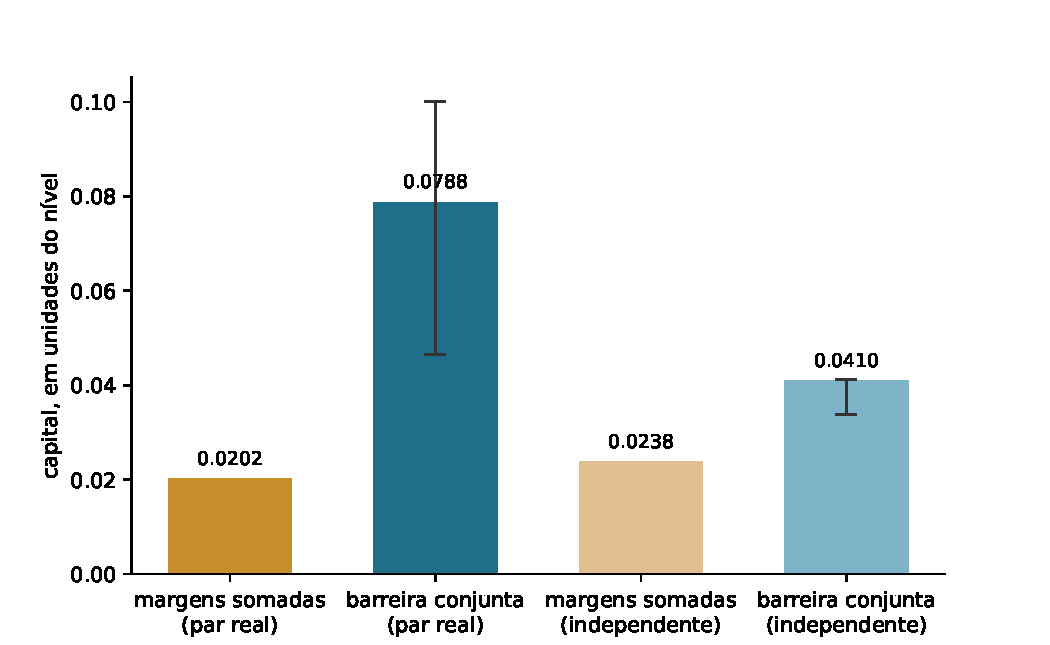
\includegraphics[width=\textwidth]{figuras/E39_preco_1.pdf}
\caption{O capital que cobre a perda da carteira no nível prometido, em unidades do nível: as
margens somadas e a barreira conjunta, no par real e nas pernas independentes, com o intervalo por
reamostragem em blocos do dia nas barras conjuntas. A barreira correta do par real custa
\numPrecoRazao{} vezes as margens somadas; nas independentes, \numPrecoIndependenteRazao.}
\label{fig:preco_contas}
\end{figure}

A carteira é declarada: metade de cada perna, nível um, o corte prometido de cinco por cento na
janela de um ano. A primeira conta é a das margens --- a mediana do corte de cada perna, participada:
\numPrecoCapitalMarginal{} do nível. A segunda é a do junto: o quantil prometido da perda da
carteira nos \numPrecoEventos{} dias em que as duas rompem o próprio corte ---
\numPrecoCapitalConjunto{} do nível, com intervalo de \numPrecoCapitalConjuntoMin{} a
\numPrecoCapitalConjuntoMax{} pela reamostragem em blocos do dia. A barreira correta custa
\numPrecoRazao{} vezes as margens somadas. E a moeda da queda conjunta confirma o buraco: de cada
dia conjunto, as margens somadas absorvem o que dá e deixam \numPrecoDescobertoMarginal{} do prejuízo
descoberto --- de \numPrecoDescobertoMarginalMin{} a \numPrecoDescobertoMarginalMax{} no intervalo.
A barreira conjunta, no seu nível prometido, deixa \numPrecoDescobertoConjunto: o desenho cobre o que
prometeu, e o que ele promete é caro.

\section{O refutador, medido}

A pergunta tem refutador declarado: se a barreira correta custar o mesmo que a errada, ela cai. Ele
não dispara no zero --- e o motivo é instrutivo. Pernas independentes com as margens do par real:
\numPrecoIndependenteEventos{} dias conjuntos, barreira a \numPrecoIndependenteRazao{} vezes as
margens, \numPrecoIndependenteDescoberto{} de descoberto. O chão não é um porque o dia conjunto já é
um dia fundo nas duas pernas --- condicionar em ambas as quedas aprofunda a perda média, mesmo sem
dependência nenhuma. Esse é o chão do aprofundamento condicional. O que a dependência cobra é a
distância dele até o par real: de \numPrecoIndependenteRazao{} a \numPrecoRazao. Mais que o dobro do
preço vem do junto --- e é exatamente a parte que a compra margem a margem não paga.

\section{A família de choque: o preço anda com o que a margem não vê}

\begin{figure}[ht]
\centering
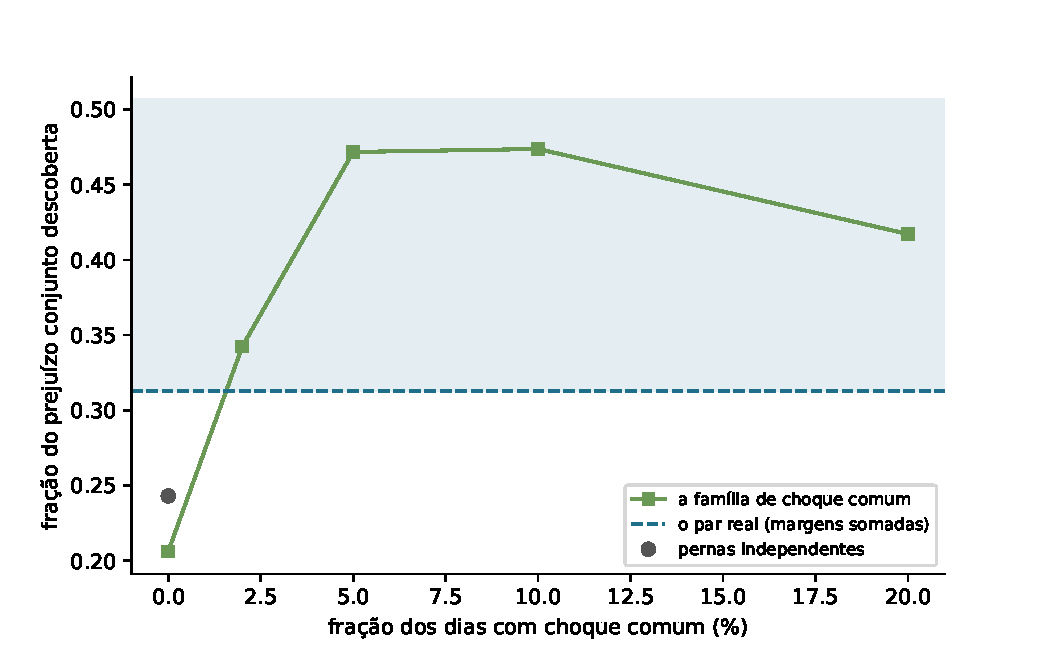
\includegraphics[width=\textwidth]{figuras/E39_preco_2.pdf}
\caption{A fração do prejuízo conjunto que as margens somadas deixam descoberta, contra a fração
dos dias com choque comum na família do capítulo da margem (com a correlação total do par,
\numPrecoRhoTotal). A linha tracejada é o par real com o seu intervalo; o ponto escuro, as pernas
independentes. O descoberto cresce com o choque e satura quando o choque deixa de ser cauda.}
\label{fig:preco_familia}
\end{figure}

Resta mostrar que o preço anda com o que o segundo momento não vê --- e a família de choque comum do
capítulo da margem é o laboratório. Com a correlação total do par declarada,
\numPrecoRhoTotal{}, a fração de dias com choque sobe do controle ao vinte por cento: o descoberto
das margens anda de \numPrecoChoqueControleDescoberto{} no controle a
\numPrecoChoqueDezDescoberto{} no dez por cento, e a razão de preços de
\numPrecoChoqueControleRazao{} a \numPrecoChoqueDezRazao. No vinte por cento ela para de subir ---
\numPrecoChoqueVinteRazao{} com \numPrecoChoqueVinteEventos{} eventos --- porque um choque que chega
a cada cinco dias deixa de ser cauda: engorda as margens tanto quanto a junta, e a razão para de
crescer. O par real, \numPrecoRazao, fica no alto da família --- entre o dez por cento e um pouco
além ---, que é a mesma leitura do capítulo da margem, agora em moeda de capital.

\section{O canal com orçamento}

Tudo o que este capítulo mediu até aqui supôs a observação completa: os dois lados da carteira vistos
no mesmo dia, todos os dias. A pergunta federada é o que sobra dessa suposição --- garantir incerteza
quando os observadores estão separados e a comunicação tem orçamento \cite{plassier2023conformal}.
O desenho é o da casa em outro material: dois canais independentes, um por perna, e só a fração
declarada dos dias atravessando cada um; o corte recalibra sobre a série que chegou, com buracos,
porque o observador não sabe o que não atravessou. O controle é embutido: com o canal aberto, os dias
comuns devolvem \numCanalVerdadeiros{} eventos conjuntos e o capital \numCanalInteiroCapital{} --- a
conta do capítulo, com a pequena diferença declarada de que a calibração agora conta só os dias
comuns.

\begin{figure}[ht]
\centering
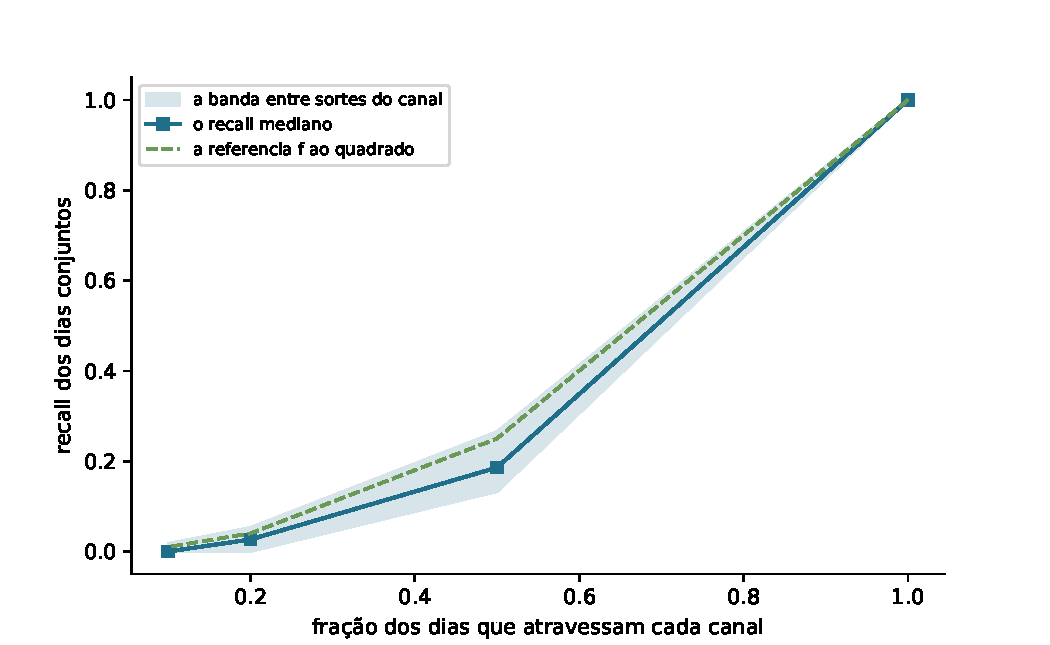
\includegraphics[width=\textwidth]{figuras/E40_canal_1.pdf}
\caption{O recall dos dias conjuntos verdadeiros contra a fração dos dias que atravessam cada canal,
com a banda entre sortes do canal --- a incerteza aqui é qual dia atravessou, e não a reamostragem dos
que vieram. A linha tracejada é a referência do quadrado: um dia conjunto só é visto se os dois canais
o deixarem passar. O recall mediano fica abaixo dela desde a metade: a recalibração sobre séries com
buracos perde além do que o canal corta.}
\label{fig:canal_recall}
\end{figure}

O canal cobra duas vezes. A primeira é o quadrado: com a metade dos dias atravessando cada canal, um
dia conjunto só é visto se ambos o deixarem passar --- e ainda assim os detectados caem para
\numCanalMeioDetectados{} [\numCanalMeioDetectadosMin{}; \numCanalMeioDetectadosMax{}] dias, com recall
de \numCanalMeioRecall{} [\numCanalMeioRecallMin{}; \numCanalMeioRecallMax{}] contra o
quarto que o quadrado previa. A segunda é a cega recalibração: o posto da janela agora conta dias
observados, o corte afrouxa ou aperta conforme o que atravessou, e o junto aparece e desaparece com a
sorte do canal. No orçamento de um quinto ela já não se sustenta: \numCanalQuintoDetectados{} dias
detectados no mediano, e a barreira conjunta só pode ser lida em \numCanalQuintoCalibraveis{} das
sortes. No décimo, o veredito é seco: zero dias no mediano, e o quantil conjunto existe em
\numCanalDecimoCalibraveis{} das sortes --- praticamente nunca.

\begin{figure}[ht]
\centering
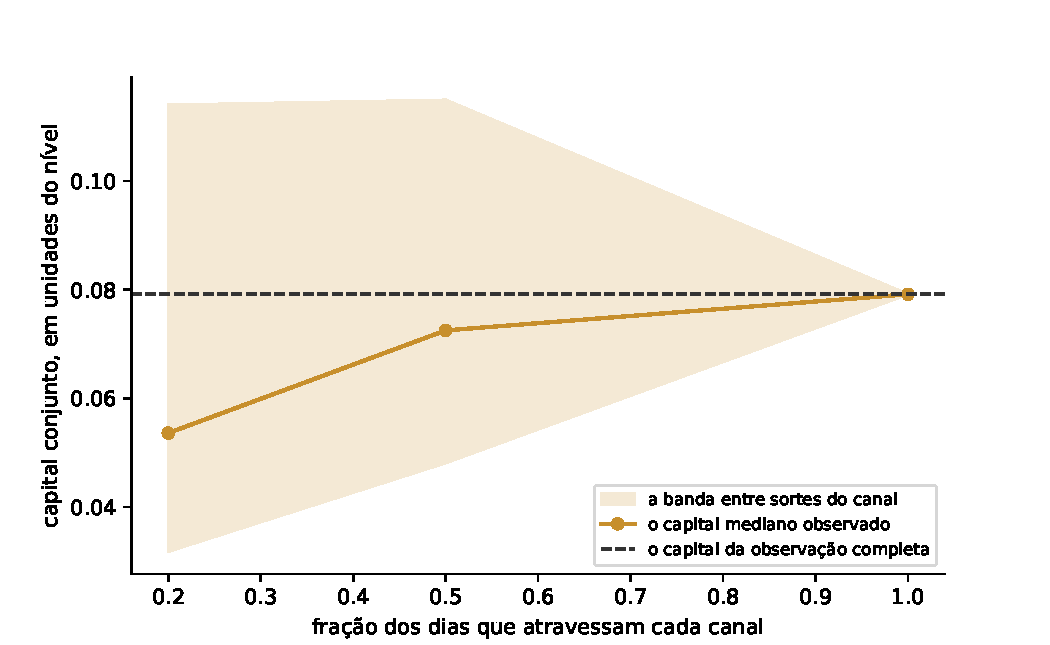
\includegraphics[width=\textwidth]{figuras/E40_canal_2.pdf}
\caption{O capital conjunto observado contra a fração do canal, nas frações em que ele pode ser lido,
com a banda entre sortes e a linha da observação completa. Na metade a banda já engole a linha: o
capital não fica mais barato --- fica ilegível. O décimo fica de fora do eixo: em quase todas as sortes o quantil nem existe ---
e o ponto do quinto só existe porque a mediana é lida nas sortes em que deu.}
\label{fig:canal_capital}
\end{figure}

E aqui está a leitura que fecha a travessia. O capítulo inteiro mediu o preço da proteção que protege
sob observação completa; o canal mostra que o preço tem um degrau antes do custo: a legibilidade. Com
a metade do orçamento, o capital mediano é \numCanalMeioCapital{} com intervalo de
\numCanalMeioCapitalMin{} a \numCanalMeioCapitalMax{} --- o número do capítulo, \numPrecoCapitalConjunto,
caído dentro da banda: nenhuma barreira calculada com metade da observação se distingue da completa.
Com menos, não há barreira que se calcule. O que não se compra tem preço, mediu o andar; o que não se
observa nem preço tem --- só a declaração honesta do orçamento que faltou.

section{O que o andar fecha}

O andar fechou pelos dois lados. De um lado, a lição com cinco nomes: nenhuma peça do livro devolve
o que a compressão jogou fora --- nem o mundo, nem o dia, nem a margem, nem a taxa, e a experiência
que provaria a causa não se compra. Do outro, a conta que este capítulo fechou: o que não se compra
tem preço mesmo assim --- \numPrecoRazao{} vezes as margens somadas, \numPrecoDescobertoMarginal{} do
prejuízo descoberto ---, e quem não o paga não está poupando capital: está devendo. A espiral vira
agora para o andar do enquadramento. Tudo o que ela mediu até aqui supôs que havia uma série, um
agora e um sistema com fronteira --- e nenhuma dessas três coisas foi discutida. Elas vêm a seguir, e
vêm porque a conta deste andar mostrou quanto custa o que fica de fora quando a fronteira é
escolhida no escuro.